\subsection{Selección Monogamica Aleatoria}
Es un mecanismo similar a la selección monogámica aleatoria, con la peculiaridad de que una vez que un individuo a sido seleccionado, no se puede volver a seleccionar en esa generación. Este algoritmo garantiza que todos los individuos se reproduzcan, sin embargo, esto podría traer el problema de que prevalezcan individuos no aptos. La Figura \ref{fig: selection_mono} muestra una representación gráfica de este proceso.

\begin{figure}[htbp]
	\centering
	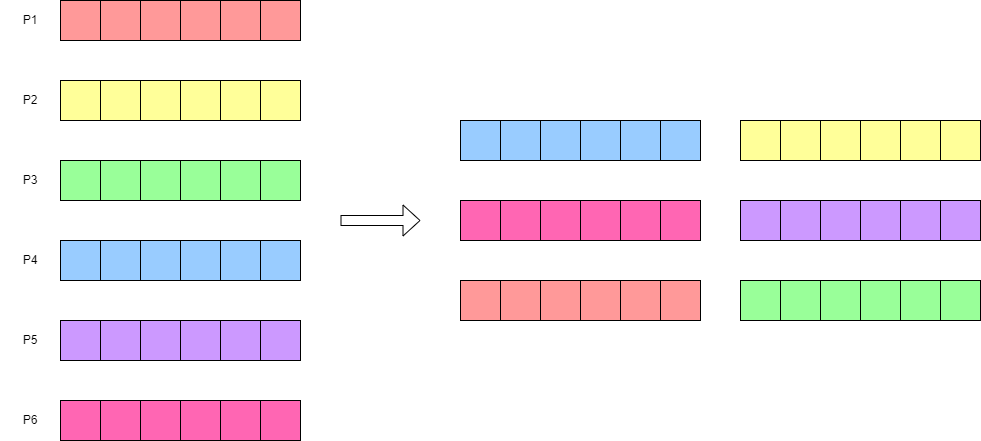
\includegraphics[width=0.8\textwidth]{random_monogamica}
	\caption{Mecanismo de selección monogámica aleatoria.}
	\label{fig: selection_mono}
\end{figure}


\subsection{Selección Torneo}
El mecanismo de selección por torneo es otro método popular utilizado en algoritmos genéticos para seleccionar individuos de una población basándose en su aptitud. Es un método relativamente simple y eficiente que puede adaptarse fácilmente para dar preferencia a individuos con mayor o menor aptitud.

La aproximación seleccionada para este trabajo consiste en realizar parejas de adentro hacia afuera dentro del conjunto de individuos. Esta aproximación presenta un problema en poblaciones grandes, ya que la diferencia de aptitud entre el individuo más alto y el menos apto es grande.

Este mecanismo se puede representar gráficamente mediante la Figura \ref{fig:TS}.

\begin{figure}[htbp]
	\centering
	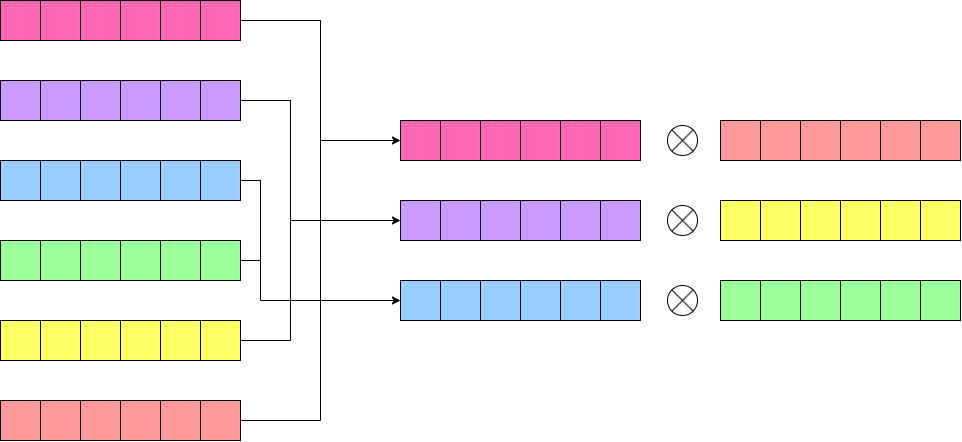
\includegraphics[width=0.8\textwidth]{tournament_selection}
	\caption{Diagrama de funcionamiento de selección por torneo.}
	\label{fig:TS}
\end{figure}


\FloatBarrier
\subsection{Cruza de un punto}
En la cruza de un punto se define un punto por el que los individuos será dividido, usualmente se escoge la mitad de estos. Una vez que se han generado los cortes, se procede a realizar una combinación cruzada de estos. La Figura \ref{fig: cross_one} muestra este proceso de forma gráfica.

\begin{figure}[htbp]
	\centering
	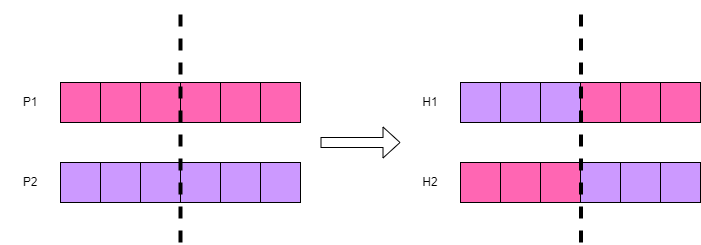
\includegraphics[width=0.8\textwidth]{crossover_one}
	\caption{Mecanismo de cruza de un punto.}
	\label{fig: cross_one}
\end{figure}


\subsection{Cruza de dos puntos}
Un proceo de cruza similar a la cruza de un punto, sin embargo, en este caso de definen dos puntos de corte y se realiza una combinación en forma de V entre los individuos. En la Figura \ref{fig: cross_two} se puede observar este proceso.

\begin{figure}[htbp]
	\centering
	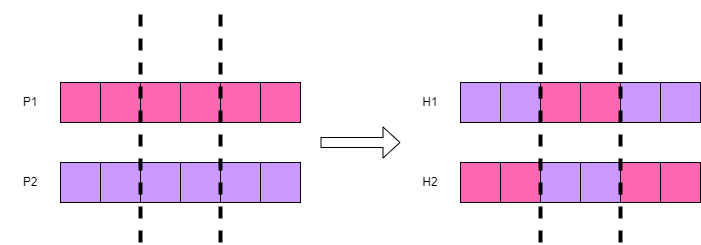
\includegraphics[width=0.8\textwidth]{crossover_two}
	\caption{Mecanismo de cruza de dos puntos.}
	\label{fig: cross_two}
\end{figure}


\subsection{Mutación Scramble}
La mutación por mezcla (scramble mutation, en inglés) es un proceso que introduce pequeños cambios aleatorios en los individuos de una población con el objetivo de aumentar la diversidad genética y explorar nuevas soluciones en el espacio de búsqueda. Dicho proceso se caracteriza por los siguientes pasos:

\begin{enumerate}
	\item Selección de un subconjunto de genes: Se elige un subconjunto aleatorio de genes en la representación del individuo. Los genes seleccionados formarán parte del proceso de mutación.
	\item Mezcla de genes: Los genes seleccionados se reordenan de manera aleatoria entre sí. Este reordenamiento aleatorio puede ser realizado de diferentes maneras, como permutando los valores de los genes dentro del subconjunto o cambiando su posición en la secuencia.
\end{enumerate}

Podemos observar una representación gráfica de este mecanismo en la Figura \ref{fig:scrM}.

\begin{figure}[htbp]
	\centering
	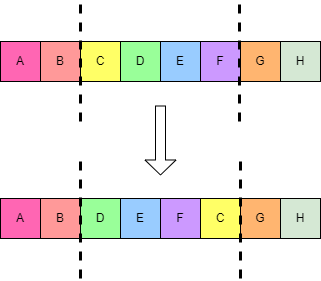
\includegraphics[width=0.4\textwidth]{scramble_mutation}
	\caption{Diagrama de funcionamiento de scramble mutation.}
	\label{fig:scrM}
\end{figure}


\FloatBarrier
\subsection{Algoritmo Multi-Islas}
Los algoritmo multi-islas implican la subdivisión de la población total en múltiples subpoblaciones, donde se ejecuta un Algoritmo Genético en cada una de ellas. Cada cierto número de generaciones, se lleva a cabo un intercambio de información entre estas subpoblaciones, conocido como migración. La introducción de la migración permite a los modelos de islas aprovechar las disparidades entre las distintas subpoblaciones, generando así una valiosa fuente de diversidad genética. Cada subpoblación se conceptualiza como una isla, y se define un procedimiento para transferir material genético de una isla a otra. La determinación precisa de la tasa de migración se revela como un aspecto crítico, ya que puede incidir significativamente en la convergencia prematura de la búsqueda.

Dentro de las diversas modalidades de comunicación entre islas, se destaca la estructura en estrella, donde se elige una subpoblación como maestra, siendo esta la que exhibe la mejor media en el valor de la función objetivo. Las demás subpoblaciones son consideradas como esclavas. En este esquema, todas las subpoblaciones esclavas envían sus mejores individuos a la subpoblación maestra, que a su vez redistribuye sus mejores individuos a cada una de las subpoblaciones esclavas. Este mecanismo establece un flujo bidireccional de información genética, fomentando la colaboración y facilitando la integración de las fortalezas individuales de cada subpoblación en el proceso evolutivo global.